\documentclass[14pt,fleqn]{extarticle}
\RequirePackage{prepwell-eng}

\previewoff

\begin{document} 
\begin{snippet}
    \correct
    
    In the figure below, the two parabolas are $y = \sqrt{2-x}$ and $y=\sqrt{x}$. And hence, the following is true 
    
    \begin{align}
	 \int_0^2 \sqrt{2-x}\cdot dx &= \int_0^2 \sqrt{x}\cdot dx \\ 
	 \therefore P &= Q 
\end{align}

\begin{center}
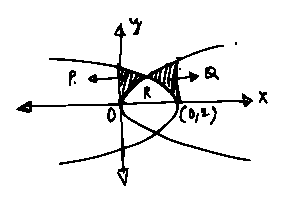
\includegraphics[scale=1.4]{figure.eps}
\end{center}
    
    
    \reason
    
    We can infer the following 
    \begin{center}
  \begin{tabular}{NNN}
   \toprule
        \text{Equation} & \text{Vertex at} & y\text{ defined if}    \\
   \midrule 
   y = \sqrt{2-x} & (2,0) & x \leq 2 \\
    \midrule 
    y = \sqrt{x} & (0,0) & x \geq 0 \\
    \bottomrule
  \end{tabular}
\end{center}

And hence we can see that 

\begin{center}
  \begin{tabular}{Nl}
   \toprule
        \text{Expression} &  Meaning \\
   \midrule 
   \int_0^2 \sqrt{2-x}\cdot dx & Area from $0\to 2 = P+R$ \\
    \midrule 
    \int_0^2 \sqrt{x}\cdot dx & Area from $0\to 2 = Q+R$ \\
    \bottomrule
  \end{tabular}
\end{center}

Moreover 
\begin{align}
\int_0^2 \sqrt{2-x}\cdot dx &= \underbrace{\int_0^2 \sqrt{2- \left(2-x \right)}\cdot dx}_{\int_0^a f(x) dx = \int_0^a f (a-x)\cdot dx} \\
&= \int_0^2 \sqrt{x}\cdot dx \\
\therefore P+R &= Q + R \\
\text{or } P &= Q 
\end{align}

\end{snippet} 
\end{document} 